\documentclass[a4paper,12pt]{article}
\usepackage[utf8]{inputenc}
\usepackage{amsmath,amssymb,amsthm}
\usepackage{natbib}
\usepackage[margin=3cm]{geometry}
\usepackage{todonotes}
\usepackage{mathtools}
\usepackage{subfiles}
\usepackage{subcaption}

%% More space between rows
\usepackage{booktabs}
\newcommand{\ra}[1]{\renewcommand{\arraystretch}{#1}}

\begin{document}
\section{Assessing the model fit}
The model uses the local past to make short term predictions about
incidence trends. As such, the performance of the model (measured
by how closely the predicted trend fits the observed trend) is
influenced by two key factors: whether the prediction is done at the
growing/declining phase of the epidemic and the length of the time
over which prediction is done.

The model fits the data well and is able to capture the strength
and direction of the trend. The analysis is computationally light
and can be carried out in real time.

The fit is particularly poor in instances where the direction of the incidence trend is reversed (i.e., case numbers start declining after a period of growth or vice versa), the model does a poor job since an underlying assumption of the model is that things will continue unchanged. This inherent shortcoming can be addressed for example by including impact of interventions in the model. However, this comes at a cost of increased complexity and requires additional data that may not be available in real-time.

Figure~\ref{fig:gf_300} shows the proportion of districts for which the
observed weekly incidence count is contained in the predicted 95\%
CI. Figure~\ref{fig:gf_500} shows the same count when the prediction
is done at 500 days. As can be seen in the two figures, in general, predictions in the short
term (2-3 weeks) are more accurate than over longer periods ($>$ 3
weeks).


  \begin{figure}
    \centering
    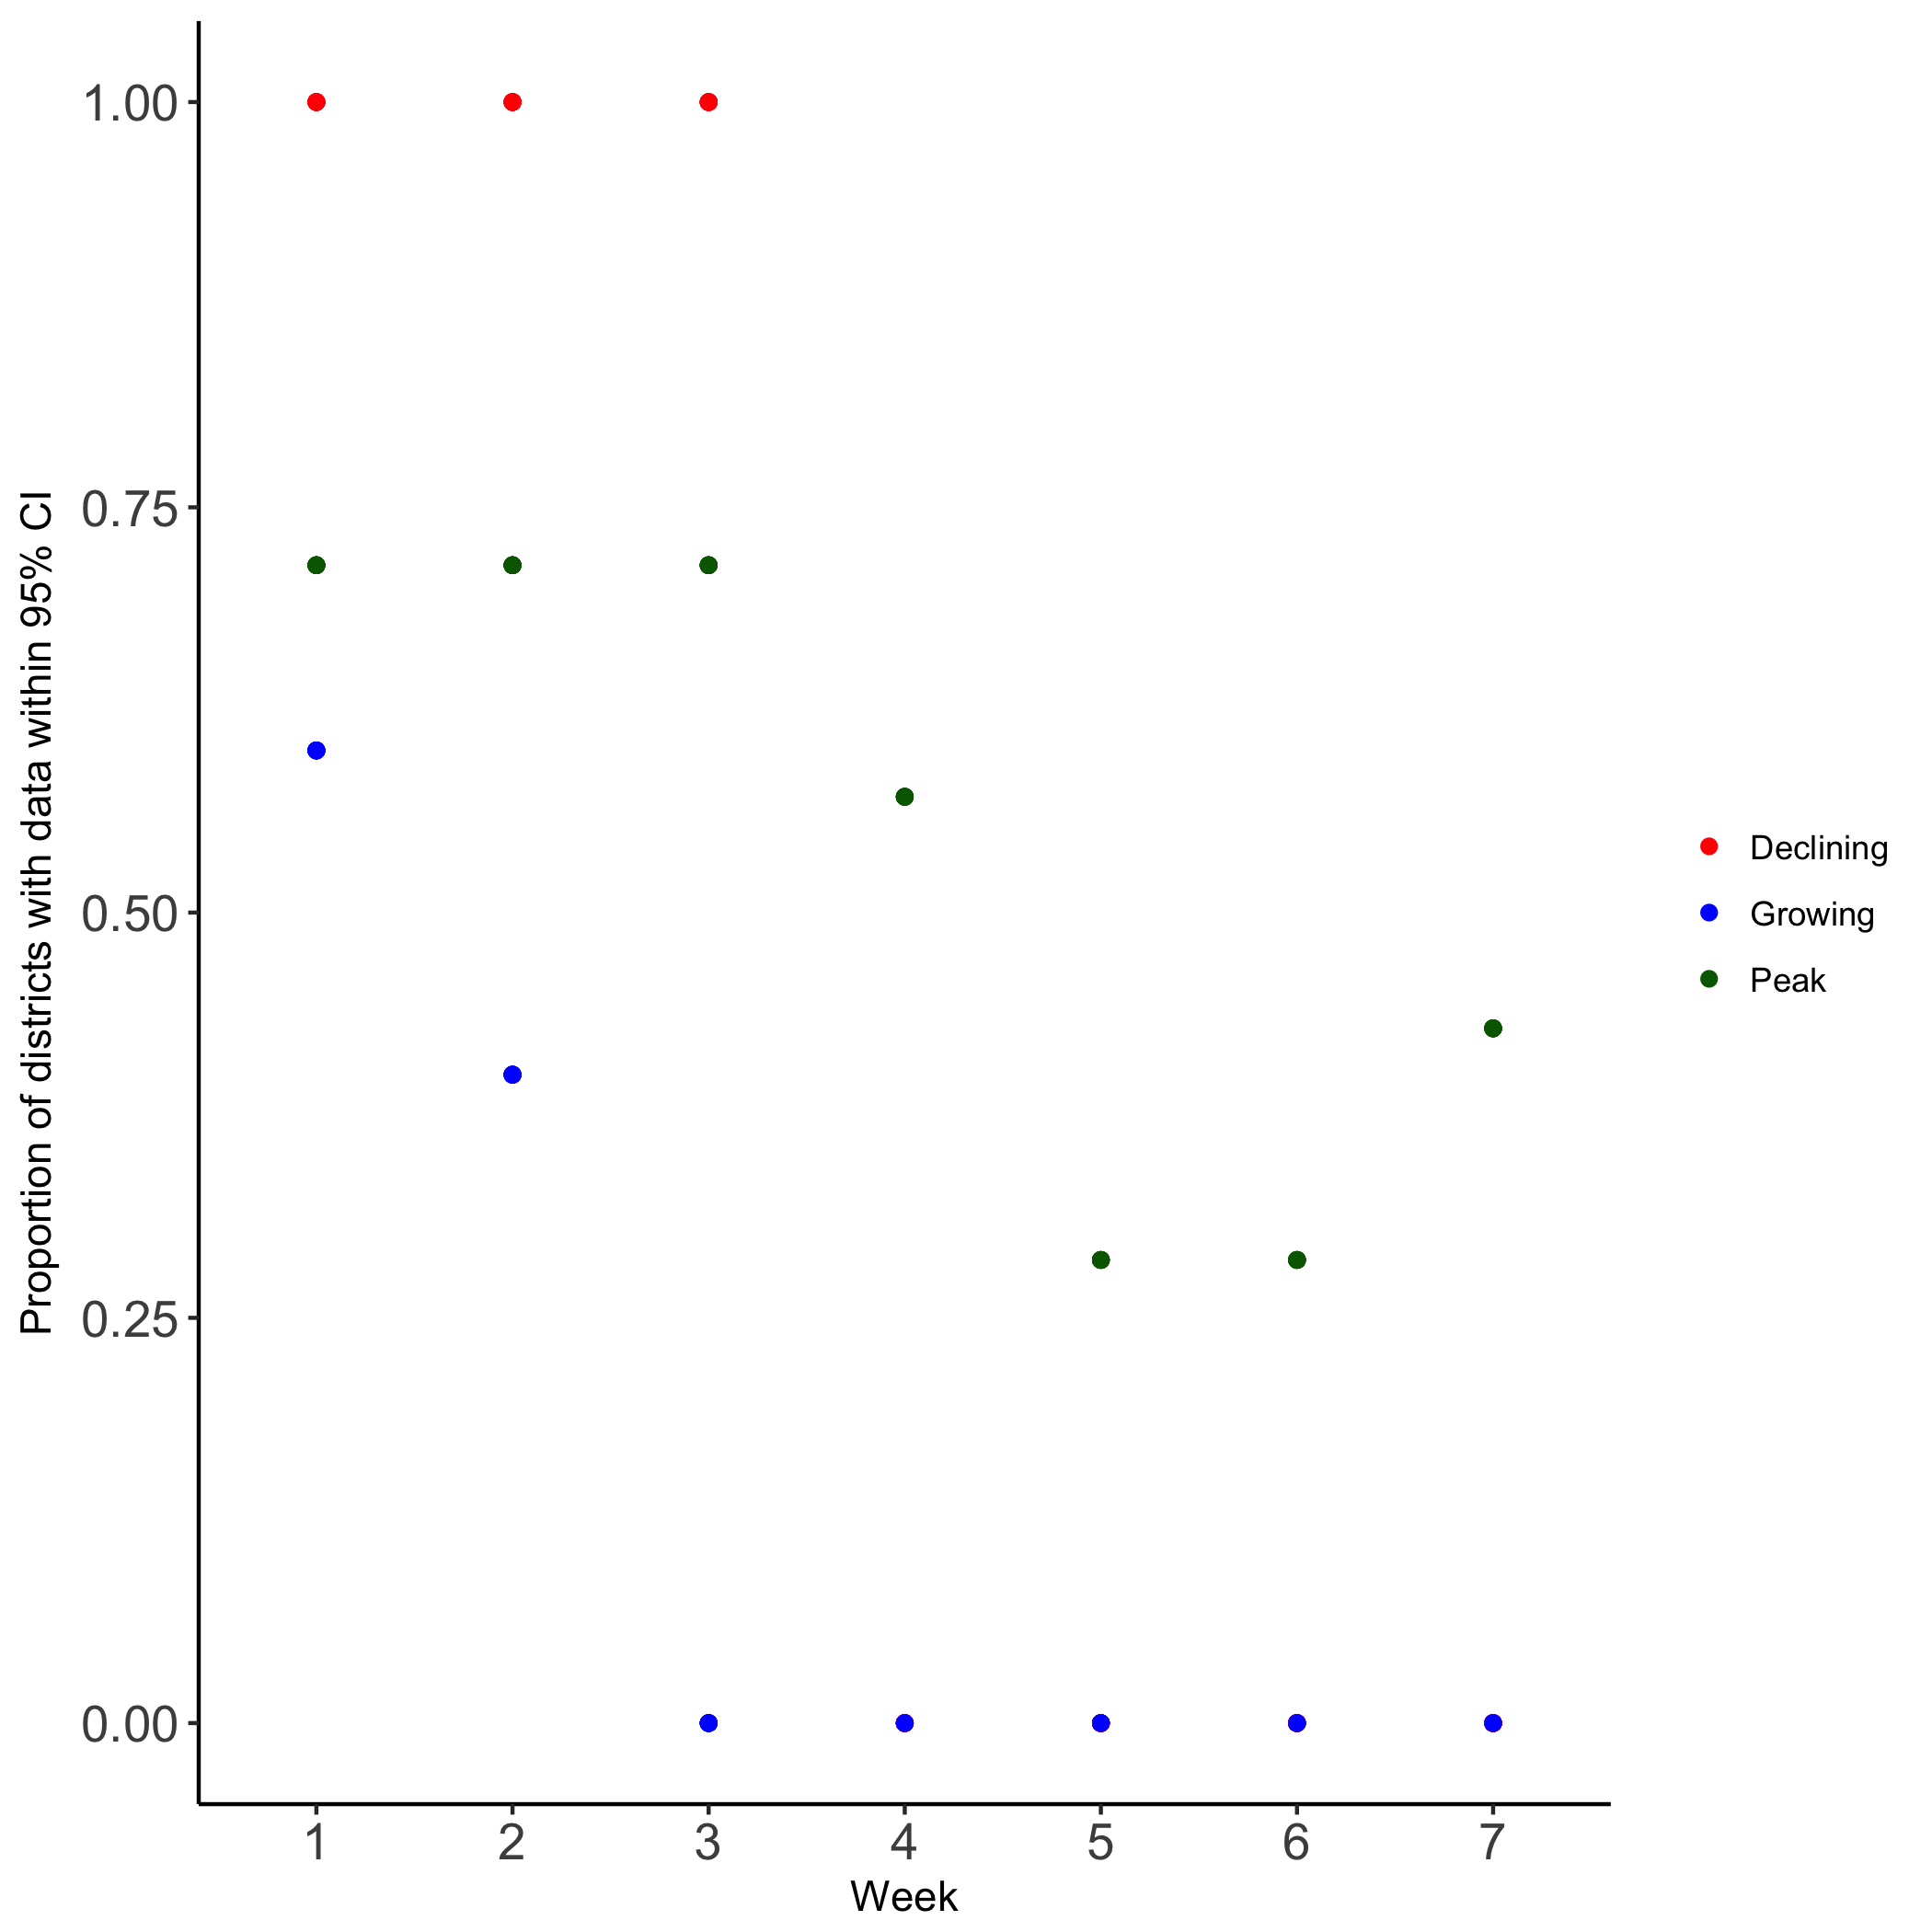
\includegraphics[scale =
    0.15]{ms6-figures/goodness_districts_300.png}
    \caption{Assessing the model fit for 7-week predictions at 300
      days. The y-axis the number of districts for which the predicted
      95\% CI contained the observed weekly incidence count. Districts
    are grouped by whether the predictions were done in a growing (R $>$
    1) or declining (R $<$ 1). If the 95\% CI of the reproduction number
    in a district in a window
  preceeding the point of prediction contains 1, the epidemic phase
  has been called ``Peak''.}
    \label{fig:gf_300}
  \end{figure}


  \begin{figure}
    \centering
    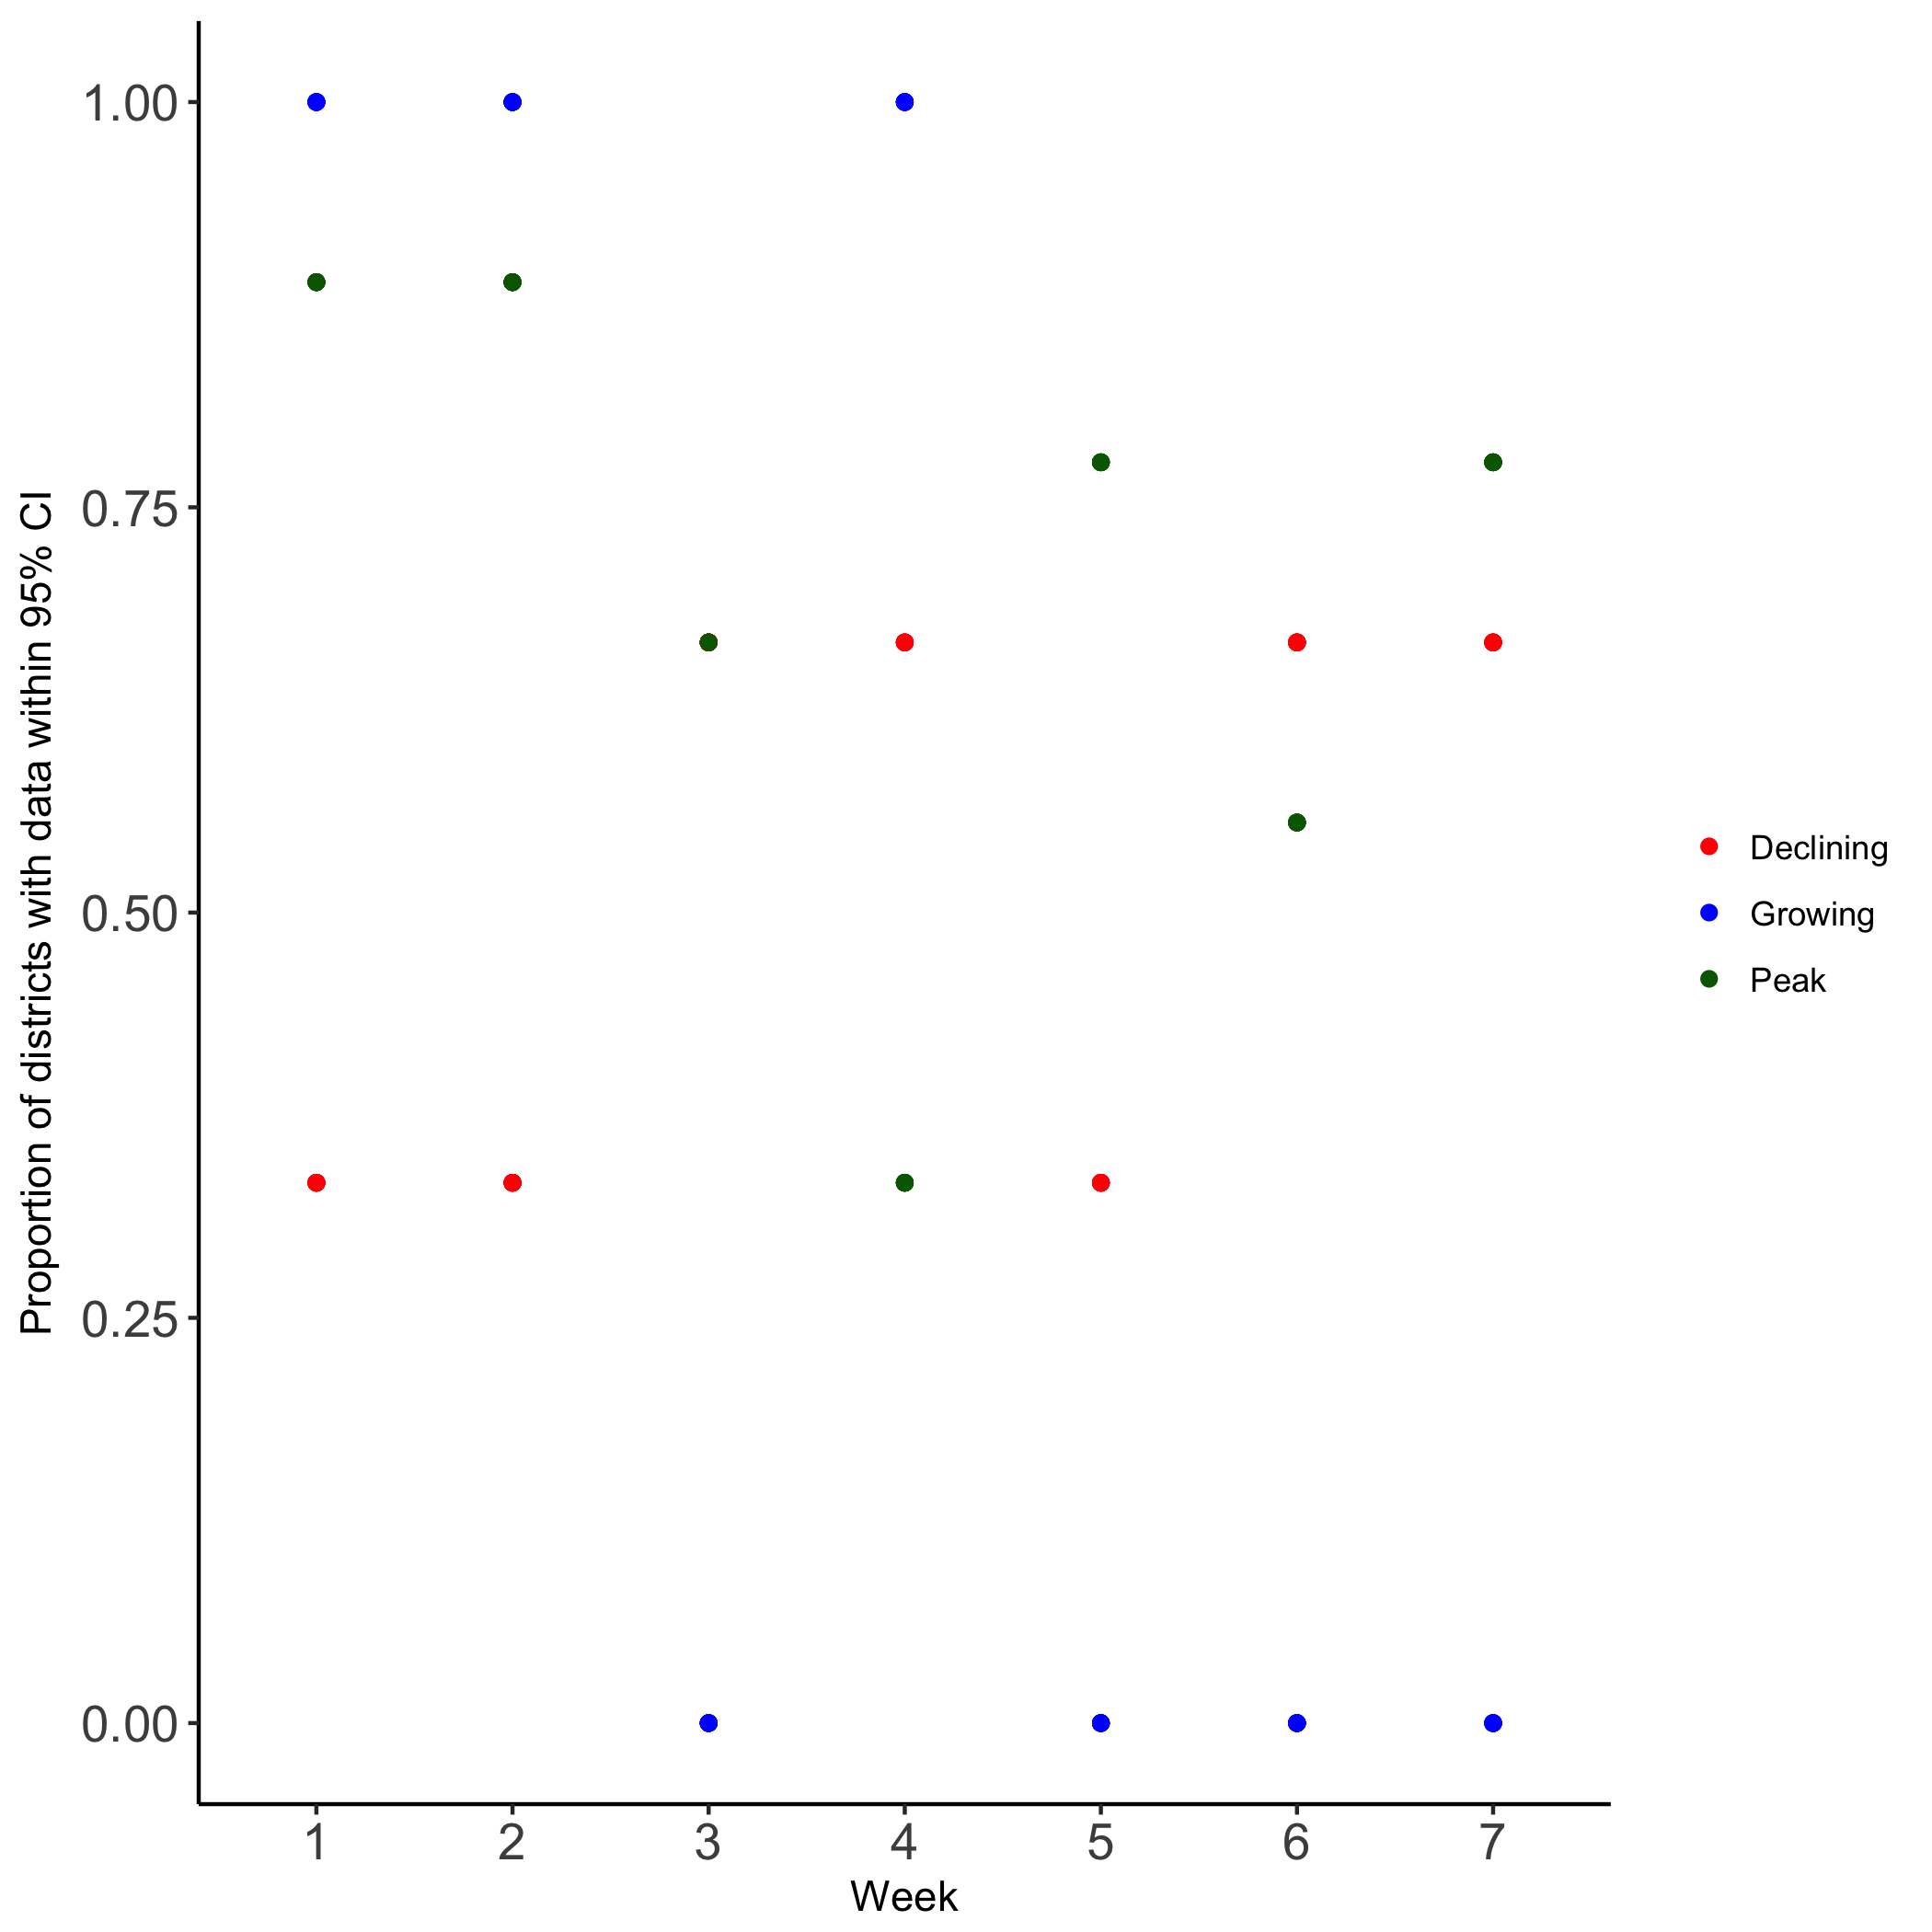
\includegraphics[scale =
    0.15]{ms6-figures/goodness_districts_500.png}
    \caption{Assessing the model fit for 7-week predictions at 300
      days. The y-axis the number of districts for which the predicted
      95\% CI contained the observed weekly incidence count. Districts
    are grouped by whether the predictions were done in a growing (R $>$
    1) or declining (R $<$ 1). If the 95\% CI of the reproduction number
    in a district in a window
  preceeding the point of prediction contains 1, the epidemic phase
  has been called ``Peak''.}
  \label{fig:gf_500}
  \end{figure}


\begin{table}\centering
  \ra{1.3}
  \begin{tabular}{@{}llr@{}}\toprule
    Phase & District & Prediction at 300 days \\
    \midrule
    Declining & Kenema & 42.9 \\
\addlinespace    
    & Bombali & 14.3 \\
    & Koinadugu & 14.3  \\    
   Growing & Port Loko & 14.3 \\
    & Tonkolili & 0 \\
    & Western & 28  \\    
\addlinespace
    & Bo &  57.1 \\
    & Bonthe &  \\
Peak    & Kailahun & 42.9 \\
    & Kambia & 28.6 \\
    & Kono & 85.7  \\
    & Moyamba & 14.3 \\
    & Pujehun & 71.4 \\
\end{tabular}
\caption{Percentage of data points (weekly incidence counts)that
lie within the predicted 95\% confidence interval. The performance of
the model ranges from poor where none of the points lie in the
interval to excellent (85\%).}
    \label{tab:fitgoodness}
  
  \end{table}
  
\end{document}